\section{Indirect Detection }

In regions of high dark matter density, dark matter particles could continue to annihilate or decay through the same process that set their relic abundance.
Of specific interest are energetic photons (i.e., X-rays and $\gamma$ rays), since photons are produced generically by the annihilation/decay of many dark matter models (either directly or as secondarily from the production of quarks or leptons). In addition, astrophysical phenomena in extreme environments could lead to conversion between Standard Model particles and the dark sector (e.g., ALPs), which could be observable through the emission energetic photons or alterations in astrophysical spectra.
By precisely mapping the distribution of dark matter and tracking extreme events (e.g. core-collapse SN) LSST will enable more sensitive searches for energetic particles originating from the dark sector.

Conventional indirect detection searches focus predominantly on WIMPs with masses between several \GeV and tens of \TeV. 
The annihilation or decay of these particles could produce energetic standard model particles detectable by current or future experiments.
The most sensitive and robust indirect searches for dark matter rely on a precise determination of the distribution of dark matter in the universe.
The integrated flux of energetic Standard Model particles $\phi_s$ (${\rm particles} \cm^{-2} \second^{-1}$), expected from dark matter annihilation in a density distribution, $\rho(\vect{r})$, is given by

\begin{equation}
   \phi_s(\Delta\Omega) =
    \underbrace{ \frac{1}{4\pi} \frac{\Gamma}{m_{\DM}^{a}}\int^{E_{\max}}_{E_{\min}}\frac{\text{d}N}{\text{d}E}\text{d}E}_{\rm particle\ physics}
    \cdot
    \underbrace{\vphantom{\int_{E_{\min}}} \int_{\Delta\Omega}\int_{\rm l.o.s.}\rho^{a}(\vect{r})\text{d}l\text{d}\Omega '}_{\rm astrophysics}\,.
    \label{eqn:indirect}
\end{equation}
%\Big\{\Big\}
\noindent Here, the ``particle physics'' term is strictly dependent on the particle physics properties---i.e., the particle mass, $m_\DM$,  the interaction rate, $\Gamma$, and the differential particle yield per interaction, $\text{d}N/\text{d}E$, integrated over the experimental energy range.
The second term, denoted ``astrophysics'', represents the line-of-sight integral through the dark matter distribution integrated over a solid angle, $\Delta\Omega$. 
For cases of dark matter annihilation, the interaction rate is set by the thermally averaged self-annihilation cross section, $\Gamma = \sigmav/2$, and the astrophysical integral is performed over the square of the dark matter density ($a=2$). 
The resulting astrophysical term is referred to as the ``\Jfactor'' \citep[\eg,][]{1998APh.....9..137B}. 
In cases of dark matter decay, the interaction rate is inversely proportional to the lifetime of the dark matter particle, $\Gamma = 1/\tau$, and the integral is performed over the dark matter density, $a=1$. 
The resulting term is known as the ``\Dfactor'' \citep[\eg][]{1408.0002}.
Qualitatively, the astrophysics term encapsulates the spatial distribution of the dark matter signal, while the particle physics term sets its spectral character. 
LSST will improve the sensitivity to dark matter particle physics by improving our understanding of the astrophysics term.
While these improvements will influence a wide range of indirect detection experiments, in this section we focus predominantly on $\gamma$-ray measurements.


\subsection{Milky Way Satellites \Contact{Andrew}}
\Contributors{Manuel M., Esra B., Andrew P., Ethan N., Alex}

\begin{figure}[t]
\centering
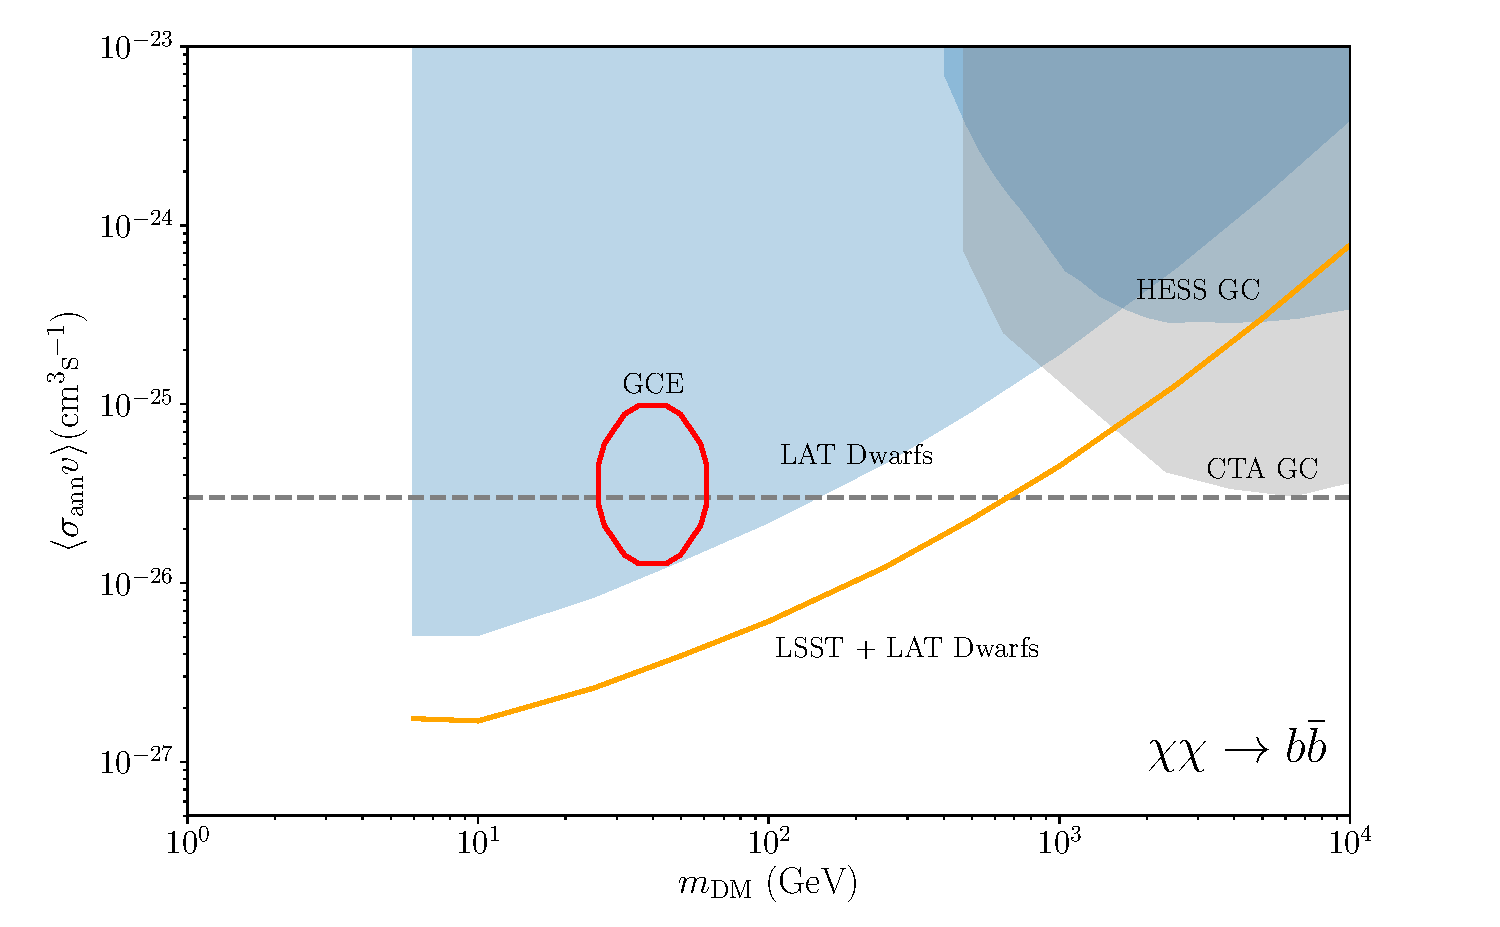
\includegraphics[width=0.75\columnwidth]{id_annih.pdf}
\caption{Constraints on dark matter annihiltion to $b\bar{b}$ from {\it Fermi-LAT} observations of Milky Way satellite galaxies \citep[LAT Dwarfs;][]{} and HESS observations of the Galactic Center \citep[HESS GC;][]{1607.08142}. 
A bracketing range of dark matter interpretations to the  Fermi-LAT Galactic Center Excess is shown in red \citep[GCE;][]{1402.6703, Gordon:2013, Abazajian:2014}.
Projected sensitivity to dark matter annihilation combining LSST discoveries of new Milky Way satellites, improved spectroscopy of these galaxies, and continued Fermi-LAT observations is shown in gold. This projection assumes 18 years of Fermi-LAT data, a factor of 3 increase in the integrated J-factor, and a factor of 2 improvement from improved spectroscopy. 
Projected sensitivity of 500h observations of the GC with CTA are shown in gray \citep[CTA GC;][]{Zaharijas:prep}.
\label{fig:indirect}
}
\end{figure}

Gamma-ray observations of Milky Way satellite galaxies currently provide the most robust and sensitive constraints on the dark matter self-annihilation cross section for GeV- to TeV-mass particles \citep[\eg][]{Ackermann:2014, Geringer-Sameth:2015, Ackermann:2015}.
The sensitivity of these searches will improve by combining new Milky Way satellite galaxies discovered by LSST, more precise $J$-factor measurements from novel spectroscopic observations, and additional Fermi-LAT data. \EN{What about CTA?}
We estimate each of these contributions to predict the improved sensitivity of dark matter annihilation searches in dwarf galaxies in the era of LSST.

To estimate the improvement in the integrated $J$-factor of the Milky Way satellite galaxy population, we combine cosmological zoom-in simulations of Milky Way dark matter substructure with a semi-analytic model to convert subhalo density profiles to $J$-factor estimates (this approach is is similar to that of \citealt{1309.4780}). 
Our simulation-based model accounts for modulations to dark matter-only subhalo populations due to baryonic physics, and we marginalize over the dependence of subhalo populations on host halo properties by sampling subhalo populations from a large number of hosts \citep{Nadler:2018}. 
To obtain an estimate for the increase to the integrated $J$-factor, we select a host halo with the largest number of nearby subhalos, consistent with recent observations of over-abundance of nearby satellites associated with the Milky Way \citep{Kim:2018, Graus:2018}. 
We exclude subhalos with heliocentric distances $< 20 \kpc$ to avoid anomalously large projections due to a single nearby satellite.
We follow the analytic formalism presented by \citet{1604.05599} and \citet{1802.06811} to convert the dark matter profiles of our simulated subhalos to \Jfactors.  
This approach estimates the \Jfactor of each subhalo based on $r_{\max}$, $V_{\max}$, and heliocentric distance. 
%We calculate the cumulative $J$-factor within 100 kpc we find for the most optimistic case 
%(i.e., selecting the host halo with the highest cumulative $J$-factor and ignoring the effects of subhalo disruption) 
We find that the cumulative \Jfactor within 100\kpc may increase by as much as a factor of 3 relative to the known dSphs with measured \Jfactors. 

Recent studies have suggested that an additional factor of 2 improvement in sensitivity may be possible through better spectroscopic measurements  of the stars in known satellite galaxies \citep{Albert:2017}, and we include this factor in our projections.
In addition, current constraints from the Fermi-LAT Collaboration used 6 years of data \citep{Ackermann:2015}; however, the Fermi-LAT has collected more than 10 years of data and could continue to collect data for another 10+ years.
These additional data will improve the statistical sensitivity of the gamma-ray search most drastically for large dark matter particle masses ($>500\GeV$).
We quantitatively evaluate the improvement from continued Fermi-LAT data taking using the results of \citep{Charles:2016}.
We combine the predicted improvements from new dwarfs, better determined $J$-factors into a projected sensitivity for future searches for dark matter annihilation in dwarf galaxies \figref{indirect}.


\subsection{Cross correlation with gamma rays \Contact{Horiuchi,Alessandro C}}
\Contributors{Horiuchi, Alessandro C}

%Wide-area weak-lensing measurements from LSST will help extract  potential dark matter contributions to the isotropic gamma-ray background \citep[IGRB;][]{1410.3696}. The IGRB is defined as the residual all-sky $\gamma$-ray emission after subtracting individually detected sources and the Galactic diffuse emission, and provides the distance frontier of indirect dark matter searches with $\gamma$ rays. Contributions to the IGRB include unresolved sources that are individually too faint to be detected---e.g., blazars \citep{1110.3787,1310.0006}, star-forming galaxies \citep{1206.1346}, and misaligned AGNs \citep{1304.0908}---as well as a potential contribution from dark matter annihilation \citep{1312.0608,1501.05464,1501.05301,1608.07289}. Analyses of the IGRB intensity spectrum, auto-correlation angular power spectrum, and photon count statistics show that a linear combination of astrophysical sources can explain the observed IGRB, but the uncertainties are still large \citep[e.g.,][]{1502.02866}.

%LSST will prove invaluable by mapping the distribution of matter on large scales via measurements of cosmic shear from weak gravitational lensing. 
%The small distortions in images of distant objects caused by gravitational lensing by the large-scale matter distribution along the line of sight is called cosmic shear. %ADW: I think this should be covered elsewhere
%Since cosmic shear and cosmological $\gamma$-ray emission from dark matter annihilation are sourced by the same underlying dark matter distribution, cross correlating them yields novel information on the composition of the IGRB \citep{1212.5018,1411.4651}. Cosmic shear unbiased tracer of dark matter distribution, which mitigates many of the systematics from using galaxies to trace dark matter---i.e., assumptions about the relationship between galaxy luminosity and halo mass, reliance on assumptions of hydrostatic equilibrium, and strong correlations with astrophysical $\gamma$-ray emission. At present, weak lensing surveys of several hundred square degrees allow studies of the IGRB to probe slightly above the thermal annihilation cross section \citep{1404.5503,1607.02187,1611.03554}. A simple forecast for LSST can be made by scaling the covariance matrix of the correlation estimator by the sky coverage. This shows that a combination of LSST lensing maps and all-sky Fermi-LAT data will reach a sensitivity where it is possible to \textit{detect} at $3\sigma$ WIMP annihilation to $b\bar{b}$ at the thermal cross cross section for up to 100 GeV masses \citep{1404.5503}. Compared to the IGRB intensity or auto-correlation, the cross correlation will yield more than $\sim 10$ times higher sensitivity to dark matter \citep{1411.4651}.  Combined cross correlations with other baryonic and gravitational tracers, e.g., galaxies and galaxy clusters \citep[\eg][]{1506.01030,Lisanti:2018,1709.01940}, will provide a better handle on the astrophysical contributors, thereby further improving sensitivity to the dark matter contribution. 
% Other references
% https://arxiv.org/abs/1411.4651

Wide-area weak-lensing measurements from LSST will help extract  potential dark matter contributions to the isotropic gamma-ray background \citep[IGRB;][]{1410.3696}. The IGRB is defined as the residual all-sky $\gamma$-ray emission after subtracting individually detected sources and the Galactic diffuse emission, and provides the distance frontier of indirect dark matter searches with $\gamma$ rays. Contributions to the IGRB include unresolved sources that are individually too faint to be detected---e.g., blazars \citep{1110.3787,1310.0006}, star-forming galaxies \citep{1206.1346}, and misaligned AGNs \citep{1304.0908}---as well as a potential contribution from dark matter annihilation \citep{1312.0608,1501.05464,1501.05301,1608.07289}. Analyses of the IGRB intensity spectrum, auto-correlation angular power spectrum, and photon count statistics show that a linear combination of astrophysical sources can explain the observed IGRB, but the uncertainties are still large \citep[e.g.,][]{1502.02866}.

LSST will prove invaluable by mapping the distribution of matter on large scales via measurements of galaxy clustering and of cosmic shear from weak gravitational lensing. 
%The small distortions in images of distant objects caused by gravitational lensing by the large-scale matter distribution along the line of sight is called cosmic shear. %ADW: I think this should be covered elsewhere
Since  cosmological $\gamma$-ray emission from dark matter annihilation also follows the same underlying dark matter distribution traced by cosmic shear and galaxies, cross correlating them yields novel information on the composition of the IGRB \citep{1212.5018,1411.4651,1506.01030,Lisanti:2018,1312.4403}. 
Compared to the IGRB intensity or auto-correlation, the cross correlation will yield more than $\sim 10$ times higher sensitivity to dark matter \citep{1411.4651,1503.05922}.
Cross-correlations with galaxy catalogs have been derived in \cite{1709.01940,1503.05918,1103.4861} up to  $z\sim 0.6$ 
which is the largest redshift where present  catalogs still have enough sky-coverage and galaxy density to robustly
detect the correlation.  On the other hand, the IGRB is expected to extend in redshift  up to $z\sim 2$--$3$ \citep{1502.02866}. 
LSST, with its large sky-coverage and galaxy density and broad redshift range, thus fills this gap to map the IGRB-LSS cross-correlation up to high redshift. 
A complete mapping of the IGRB up to $z\sim3$ will constitute a crucial tool to robustly separate the different 
astrophysical contributions, as well as to isolate the DM annihilation signal, breaking the degeneracies which
are present when only low redshift results are used \citep{1506.01030}.    

Complementary to galaxy catalogs, cosmic shear has the advantage of being an unbiased tracer of dark matter distribution, which mitigates many of the systematics from using galaxies to trace dark matter---i.e., assumptions about the relationship between galaxy luminosity and halo mass, reliance on assumptions of hydrostatic equilibrium, and strong correlations with astrophysical $\gamma$-ray emission. At present, weak lensing surveys of several hundred square degrees allow studies of the IGRB to probe slightly above the thermal annihilation cross section \citep{1404.5503,1607.02187,1611.03554}. A simple forecast for LSST can be made by scaling the covariance matrix of the correlation estimator by the sky coverage. This shows that a combination of LSST lensing maps and all-sky Fermi-LAT data will reach a sensitivity where it is possible to \textit{detect} at $3\sigma$ WIMP annihilation to $b\bar{b}$ at the thermal cross cross section for dark matter particle masses up to 100 GeV \citep{1404.5503}.   

%Combined cross correlations with other baryonic and gravitational tracers, e.g., galaxies and galaxy clusters \citep[\eg][]{1506.01030,Lisanti:2018,1709.01940}, will provide a better handle on the astrophysical contributors, thereby further improving sensitivity to the dark matter contribution. 
% Other references
% https://arxiv.org/abs/1411.4651


From the gamma-ray side, improvements in the mapping of the cross-correlation with galaxies and cosmic shear are expected with the foreseen new generation gamma-ray instruments AMEGO\footnote{\url{https://asd.gsfc.nasa.gov/amego/index.html}} and eASTROGAM\footnote{\url{http://eastrogam.iaps.inaf.it/}} \citep{1711.01265}.
At the present, the main limitation in detecting the cross-correlation at GeV and sub-GeV energies is the angular resolution, rather than the available statistics.  
eASTROGAM, in particular, will have in the energy range \mbox{100 MeV-1 GeV} an angular resolution 5-6 times better than Fermi-LAT~\citep{1711.01265}. This will translate in harmonic space into a multipole reach 5-6 times larger than presently achievable, and as a consequence stronger constraints from the cross-correlation.
Precise measurements of the cross-correlation at sub-GeVs will further improve the ability to separate the astrophysical IGRB sources from the DM signal, increasing the sensitivity to the latter. 


\subsection{Axion-like particle emission from supernovae \Contact{Manuel}}
\Contributors{Manuel, ...}

Axion-like particles (ALPs) might be produced during core-collapse supernova explosions through the conversion of thermal photons in the electro-static fields of protons and ions, i.e., through the Primakoff effect \citep{1996slfp.book.....R}.  
Similar to neutrinos, ALPs would quickly escape the core and, if they are sufficiently light ($m_\phi \lesssim 10^{-9}\,$eV), they could convert into $\gamma$~rays in the magnetic field of the Milky Way and/or the host galaxy of the core-collapse supernova. 
The resulting $\gamma$~rays would arrive in temporal coincidence with the neutrinos in a burst lasting tens of seconds with a 
thermal spectrum peaking 60\MeV, depending on the mass of the progenitor \citep{2015JCAP...02..006P}.
The non-observation of a $\gamma$-ray burst from the SN1987A, which occurred in the Large Magellanic Cloud, has been used to derive stringent constraints on the photon-ALP coupling $g_{\phi\gamma}<5.3\times10^{-12}\GeV^{-1}$ for $m_\phi < 4.4\times10^{10}\eV$ \citep{1996PhLB..383..439B, 1996PhRvL..77.2372G,2015JCAP...02..006P}.
In the case of a core-collapse supernova within the Milky Way, the \textit{Fermi} LAT could improve these limits by more than an order of magnitude \citep{2017PhRvL.118a1103M}. 
However, with a Galactic supernova rate of $\roughly 3$ per century \citep[e.g.,][]{2013ApJ...778..164A}, and the LAT field of view of 20\% of the sky, the chance to observe at least one such event in the next five years is $\sim 0.03 \cdot 0.2 \cdot 5 = 0.03$ assuming that the occurrence of supernovae is a Poisson process. This estimate is still optimistic since the supernova rate is calculated for the entire Galaxy, which is not inside the field of view at any given moment.\footnote{If the supernova is sufficiently close-by or the photon-ALP coupling is close to current limits, a signal could be detected with the BGO detectors (senisitive up to 40\,MeV) of the \emph{Fermi} Gamma-ray Burst Monitor, which observes the entire unocculted sky.}
Increasing the search volume to extragalactic supernova is the obvious way to overcome this low rate. 
However, for core collapse SN beyond the LMC and SMC, current-generation neutrino detectors lack the sensitivity to detect a signal \citep[e.g.,][]{2011PhRvD..83l3008K}, and hence no precise time stamp will be provided for ALP-induced $\gamma$-ray emission, however, well-sampled optical light curves can be used to estimate the explosion time on the time scale of hours \citep{2010APh....33...19C}. 
LSST will detect a plethora of core-collapse supernova light curves \citep{Lien:2009}. 
Estimates for the delay between the core collapse and the shock breakout range from minutes for massive Wolf-Rayet stars (supernova of type Ib/c) to days for red supergiants (type II supernovae) \citep{2013ApJ...778...81K}. 
Thus, type Ib/c supernova caught early after their shock breakout and with subsequently well sampled light curves are a prime target for the search of an ALP-induced $\gamma$-ray burst. 

Since the $\gamma$-ray flux scales as $g_{\phi\gamma}^4 / d^2$, where $d$ is the luminosity distance, the sensitivity for $g_{\phi\gamma}$ scales as $\sqrt{d}$. 
Limits of the order of $g_{\phi\gamma} \lesssim 2\times10^{-12}\,\mathrm{GeV}^{-1}$ should be possible for a single supernova in M31 ($d=778$\,kpc) \citep{2017PhRvL.118a1103M}. 
If one allows these limits to degrade by a factor of 10, constraints better than the ones from CAST should still be possible for $d\lesssim 80\,$Mpc ($z \lesssim 0.02$) for a single supernova assuming that the time of the core collapse is known. 
LSST is expected to detect tens of type Ib/c core-collapse supernovae every year with redshifts $z \lesssim 0.02$ \citep{Goldstein:2018} and could conduct such searches in conjunction with the \textit{Fermi} satellite or future $\gamma$-ray satellites like AMEGO, eASTROGAM, or Gamma-400 \citep[\eg,][]{2017ICRC...35..910C,1502.02976} 
%(EN Gamma-400?). \ADW{I think the high-energy field of view of Gamma-400 is probably too small to make this compelling, but the GRB system could be interesting up to 15 MeV.}
%LSST is expected to detect more than $10^4$  core-collapse supernovae every year with redshifts $z \lesssim 0.1$ \citep{2009JCAP...01..047L} and is therefore an excellent instrument to conduct such searches in conjunction with the \textit{Fermi} LAT or future $\gamma$-ray satellites like AMEGO or eASTROGAM \citep[see, e.g.,][]{2017ICRC...35..910C}. 
A stacking analysis of the $\gamma$-ray data with explosions times estimated from LSST light curves provides the exciting possibility to photon-ALP couplings in the regime where ALPs could make up the entirety of the dark matter. 


%\subsubsection{Transient Objects \Contact{???}}
%\Contributors{Renee?, Chanda, Esra, Manuel M., ... }

%From Chanda PW and Esra B: 
%\ADW{This is an X-ray cross-correlation paragraph written by Chanda and Esra. I think we would need a more quantitative estimate to include it in the discussion. Out to what distance would these KN be detected? How good would the timing need to be? etc.}
%The wide-fast-deep LSST survey will be uniquely positioned to detect up to 10 kilonovae per year (LSST Science Book 2009, Rosswog et al. 2016). These detections can be combined with timing data from those sources from ongoing X-ray experiments such as NICER (and proposed experiments such as STROBE-X and IXPE) can be used to search for proposed axion cooling tracks (Keller and Sedrakian 2013, Sedrakian 2016), leading to constraints on the axion parameter space. 

%LIGO/kilonova connection for optical follow-up?
%\TT{I could write something here re LSST followup}
% ADW: Probably a better estimate of the kilonova rate (3 - 6 per year) 
% ADW: Rough estimate for the kilonova rate (75 - 2200 like GW170817 within z ~ 0.25) from Section 7.1 of 1809.04295
